\section{Problem}
There are several sub-problems in a system of this nature that the project needs to address.

\begin{itemize}
\item Decentralization of of system logic
\item Source code integrity
\item Peer identity verification
\item Resource storage
\item Resource identification
\item Distribution and storage of cryptographic keys
\item Communication flow and transfer initiation
\end{itemize}

Below, these main points affecting the architecture are presented.

\subsection{Decentralization of system logic}
In a truly distributed system, it is necessary to avoid having crucial system logic and data on a server. The functionality of the system should not rely on availability any central server. Temporary downtime can be accepted as long as servers do not store crucial data and can be replaced with new servers running the same software. Since clients can not know what application their peers are running, all information from other peers must be verified and considered as untrusted.

\subsection{Source code integrity}
Since the system logic is run in a web browser, how can one trust the fact that the client code is not altered between executions? This issue is one of the reasons why a large part of the online community is considering client-side JavaScript encryption to be a generally bad practice. At the time of this writing, major web browsers have no way to verify client-side code or resources the way that native binaries or Java applets can be cryptographically signature checked.

\subsection{Peer identity verification}
Each user of the system will be associated with a self-generated private-public pair of cryptographic RSA keys. With knowledge of the public keys of their peers, there are standardized identity verification protocols used on a session-to-session basis. Regardless of the authentication protocol used, there is always a chicken-and-egg problem with the distribution of public keys and how to tie them to identities. Traditionally, there are two types of Public Key Infrastructures (PKIs) with different ways to address this:

\begin{itemize}
  \item A Web of Trust, as often utilized in OpenPGP \cite{Maurer:1996}. Here, a user has a list of peers that they trust - trusted introducers. If they receive a public key and associated identity signed by one of their trusted introducers, they will know that the trusted introducer has verified the connection between the identity and the public key. This way, an active user will steadily grow their network of trusted introducers. One needs to have a network of dependable and active peers in order to successfully participate in a Web of Trust.
\item A PKI centered around one or several Certificate Authorities (CAs). Here, there is a predefined list of authorities that are trusted to sign participants public keys. This creates a centralized network and puts a lot of trust in the CAs. SSL utilizes this approach and there are several historical examples of when this trust has been broken (more recently in the Diginotar hack of 2011).
\end{itemize}

For a truly decentralized system, it is not acceptable to adapt a CA-entered approach. While a Web of Trust is interesting, it might be too cumbersome for users. This issue is addressed in “Zooko’s Triangle” (See figure \ref{fig:zooko}), stating that no system assigning names to participants in a network can have the property that names are secure, decentralized and meaningful at the same time. This conjecture has since been proven false by the design of systems such as the blockchain of the cryptocurrency Namecoin, which effectively acts as a cryptographically secured distrubuted hash table (DHT) with unique keys.

\begin{figure}[h]
\centering
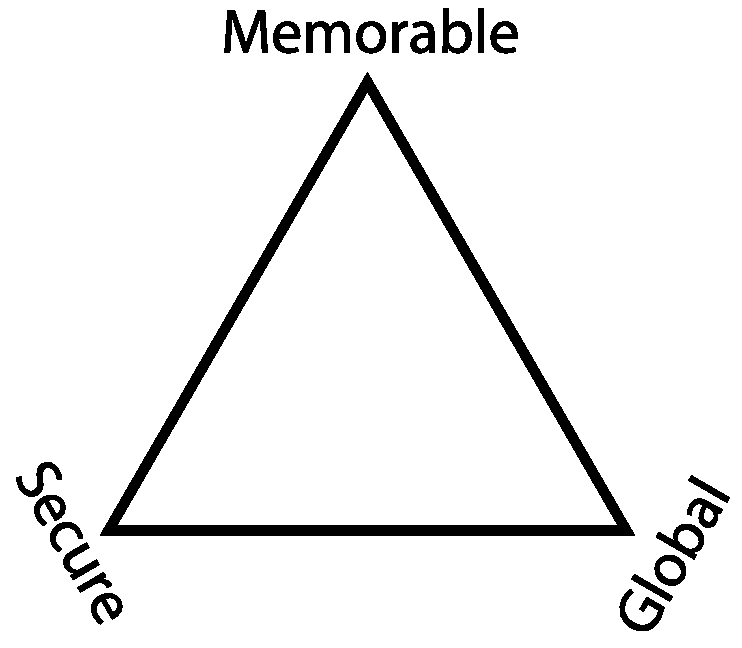
\includegraphics[width=\textwidth,height=0.2\paperheight,keepaspectratio
]{figures/Zooko_s_Triangle}
\caption{Zooko's Triangle, with the edges representing the achievable combinations of features \cite{Zooko:2001:Online}}
\label{fig:zooko}
\end{figure}

\subsection{Resource storage}
Usability, security and adherence to public web standards are three priorities that make the question of how to locally store resources on clients a difficult one. There are proprietary technologies for mapping resources to files on the local filesystem, which could be very useful – but without cross-platform support, it is considered out of the question.

\subsection{Resource identification}
It is desirable for resources to have identifiers that are both memorable, secure, and unique - Zooko’s triangle is a concern here as well. However, there are practical limitations on using any current cryptocurrency blockchain here. There is a monetary cost associated with the insertion of a new value, and updates can take a significant amount of time to propagate over the network. These practical issues would make such a system practically unusable. File names are not even close to unique and disclose unnecessary information, should an adversary without the corresponding secret key get hold of an encrypted resource. Since resources are communicated peer-to-peer, the issue of malicious resource identifier collision attacks becomes negligible since users would have first-hand contact with peers that they trust and can verifiy the identity of. Resource checksums will have to be communicated and verified by peers before accepting a transfer of resource data.

\subsection{Distribution and storage of cryptographic keys}
Assuming that the system can utilize a DHT such as a cryptocurrency blockchain for storage of the public part of RSA key pairs, the issue of how to interface a web application with the blockchain in a way that allows for verification of identities without putting too much trust in the HTTP/cryptocurrency gateway also needs to be addressed. Additionallyl, as previously stated, the initial insertion of the key requires monetary resources, and is perhaps something that should be solved outside of Rymd.
While the public key can be stored in a DHT, private keys need to be stored securely on each client, preferably without giving client code any direct access to the raw keys. How the initial generation of keys are performed also needs consideration. Finally, a secure way to store the encryption keys for encrypted resources needs to be addressed. The question of how these resource-associated secret keys are distributed is deemed an implementation-specific question and will be out of scope for Rymd, but handled in Shuttle.

\subsection{Communication flow and transfer initiation}
Once peers have verified each other’s identities, the question of how two peers start the transfer of a shared resource arises. This is also an implementation detail in applications using the library and depends on what problems that particular application is intending to solve.

